\section{着色方程}

\subsection{着色方程的建立}
我们考虑\xref{fig:着色原理}所示的着色过程示意图,先将所有符号说明如下
\begin{itemize}
    \item Light表示点光源的位置,在本节考虑的光源暂且都是点状的。
    \item View表示视线原点的位置。
    \item 向量$\vb{n}$代表三角面朝外的的单位法向量。
    \item 向量\hspace{0.47em}$\vb{l}$\hspace{0.47em}代表三角面(与视线交点处)指向光源点的单位向量。
    \item 向量$\vb{v}$代表三角面(与视线交点处)指向视线原点的单位向量。
    \item 向量$\vb{h}$代表指向$\vb{v},\vb{l}$角平分线的单位向量,可由$\vb{h}=(\vb{v}+\vb{l})/\norm{\vb{v}+\vb{l}}$得到。
\end{itemize}
\begin{Figure}[着色原理]
    \begin{FigureSub}[Lambertian着色]
        \includegraphics[scale=0.8]{build/Chapter09A_01.fig.pdf}
    \end{FigureSub}\hspace{0.5cm}
    \begin{FigureSub}[Blinn-Phong着色]
        \includegraphics[scale=0.8]{build/Chapter09A_03.fig.pdf}
    \end{FigureSub}\\ \vspace{0.5cm}
    \begin{FigureSub}[Ambient着色]
        \includegraphics[scale=0.8]{build/Chapter09A_02.fig.pdf}
    \end{FigureSub}
\end{Figure}

着色过程可以分成以下三种机制:Lambertian着色、Blinn-Phong着色、Ambient着色。
\begin{BoxFormula}[Lambertian着色]
    Lambertian着色表征了点光源的漫反射
    \begin{Equation}
        c=c_lc_d\max(0,\vb{n}\cdot\vb{l})
    \end{Equation}
\end{BoxFormula}
\begin{BoxFormula}[Blinn-Phong着色]
    Blinn-Phong着色表征了点光源的镜面反射
    \begin{Equation}
        c=c_lc_s\max(0,\vb{n}\cdot\vb{h})^p
    \end{Equation}
\end{BoxFormula}
\begin{BoxFormula}[Ambient着色]
    Ambient着色表征了环境光源的漫反射
    \begin{Equation}
        c=c_ac_d
    \end{Equation}
\end{BoxFormula}

这三种着色机制是共同作用的,最终的着色结果是三者之和
\begin{Equation}
    c=c_ac_d+c_lc_d\max(0,\vb{n}\cdot\vb{l})+c_lc_s\max(0,\vb{n}\cdot\vb{h})^p
\end{Equation}

接下来,我们将逐步解读这三种着色机制对应的着色方程的物理意义及相关符号的含义。

\subsection{着色方程的意义}

第一步,我们要理解光源照射至物体表面时,存在两种光学过程
\begin{itemize}
    \item 漫反射(Diffuse Reflection):光线照射至粗糙表面时会由于表面的不平整而向各个方向反射。这就是说,漫反射向各个方向均匀反射了从光源吸收的能量,因而从任意角度看表面都是完全相同的亮度,换言之,漫反射是视角无关的!那么,漫反射下表面的亮度与什么有关?朴素的观察指出,光垂直照射表面是最亮的,光平行照射表面是最暗的,在数学上,这可以用表面法向量$\vb{n}$与光线向量$\vb{l}$的夹角余弦$\cos\theta$表示,我们可以简单验证这一点:垂直照射$\theta=0$时有$\cos\theta=1$,平行照射$\theta=\pm\pi/2$时有$\cos\theta=0$。当然必须要考虑到的是,亮度不可能小于零,当光线照向了表面的背面时不可能“比黑更黑”,故修改为$\max(0,\cos\theta)$。最后,由于$\vb{n},\vb{l}$均为单位向量,因此可以改写为$\max(0,\vb{n}\cdot\vb{l})$。
    \item 镜面反射(Specular Reflection):光线照射至较光滑的表面时反射光线会相对集中在镜面反射方向上。换言之,如果视线恰好在反射方向附近,我们将看到更亮的光。而考察视线和反射方向是否重合,其实等价于考察视线和光线的角平分线方向$\vb{h}$是否位于表面法向$\vb{n}$上,因而有了$\max(0,\vb{n}\cdot\vb{h})$,添加一个系数$p>1$即$\max(0,\vb{n}\cdot\vb{h})^p$可以使视线偏离反射方向后亮度以更快的速度衰减至零。系数$p$反映了表面的光滑程度,系数$p$较大则意味着表面较光滑,使反射光线只集中在镜面反射方向附近的一个很小的角度范围内。
\end{itemize}

其中,Lambertian着色和Blinn-Phong着色分别代表了点光源的漫反射和镜面反射。然而若仅考虑这两者会导致一个问题,即背朝光源的表面将是完全黑暗的,这不美观也不符合我们的实际感受。Ambient着色引入了环境光源,环境光源可以认为是弥散在整个环境中各向同性的光源,换言之,环境光源对于每一个表面都是垂直照射的,保障一个最低程度的照明。

第二步,我们要理解方程中各颜色$c_l,c_a,c_d,c_s$的含义,所有颜色可以分为两组
\begin{itemize}
    \item 光源颜色$c_l,c_a$\hspace{0.15em}:分别代表“点光源颜色”和“环境光源颜色”。
    \item 物体颜色$c_d,c_s$:分别代表“漫反射颜色”和“镜面反射颜色”。
    \item 有关符号下标,$c_l,c_a$代表Light和Ambient,$c_d,c_s$代表Diffuse和Specular。
\end{itemize}
而对于一种着色机制,取决于光源类型和反射机制,会带有两项颜色系数
\begin{itemize}
    \item Lambertian着色是点光源的漫反射,故有$c=c_lc_d\max(0,\vb{n}\cdot\vb{l})成立$。
    \item Blinn-Phong着色是点光源的镜面反射,故有$c=c_lc_s\max(0,\vb{n}\cdot\vb{h})^p$成立。
    \item Ambient着色是环境光源的漫反射(环境光总垂直表面),故有$c=c_ac_d$成立。
\end{itemize}

应当指出,这里$c_l,c_a,c_d,c_s$都应该解读为颜色的某一分量,完整的结果需对于RGB的每一颜色分量重复一遍。这是符合直觉的,白色的光照射在红色物体上我们将只会看到红色。


还要注意的是,由于$c\in[0,1]$,为了保证$c$的结果不溢出该范围,需要加一些限制。

光源颜色的总和不能超过$1$
\begin{Equation}
    c_l+c_a\leq 1
\end{Equation}
物体颜色的总和不能超过$1$
\begin{Equation}
    c_d+c_s\leq 1
\end{Equation}
这里我们可能对$c_d+c_s\leq 1$带来的物体颜色无法自由指定感到困惑。但可以这么想,若一个物体需要表现出高光,那它本身的颜色就不可能太亮,否则高光部分又怎么显示出“高光”呢?

注意,Lambertian和Blinn-Phong均为人名,但Ambient不是,它的意思就是环境!

\subsection{着色方程的效果}
\paragraph{Lambertian着色}
\xref{fig:Lambertian着色}展示了Lambertian着色的效果,该球自身为灰色,场景中使用了两个点光源,左上方设置了一个较亮的白色点光源,右侧设置了一个较暗的蓝色点光源,两者的效果是叠加的。
\begin{Figure}[Lambertian着色]
    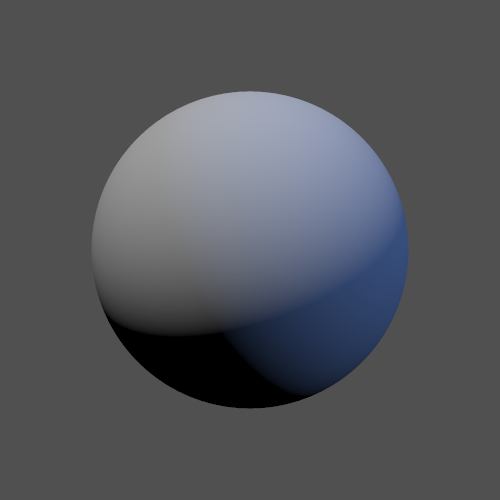
\includegraphics[width=6.5cm]{image/RasterizationIOW/SphereLambertian.png}
\end{Figure}

\paragraph{Ambient着色}
\xref{fig:Ambient着色}展示了Ambient着色的效果,环境光的引入使阴影部分也有一定亮度。
\begin{Figure}[Ambient着色]
    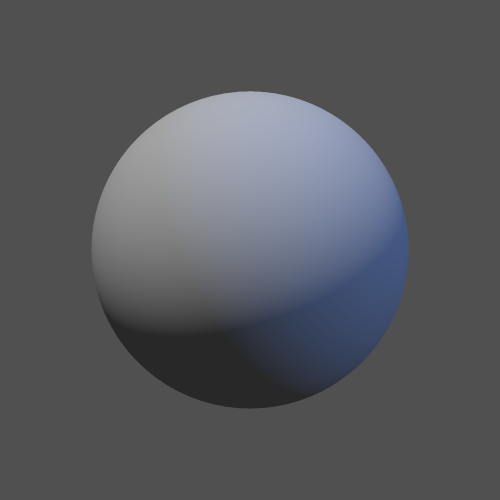
\includegraphics[width=6.5cm]{image/RasterizationIOW/SphereAmbient.png}
\end{Figure}

\paragraph{Blinn-Phong着色}
\xref{fig:Blinn-Phong着色}展示了Blinn-Phong着色的效果,注意到两个光源在球面上形成的高光。

\begin{Figure}[Blinn-Phong着色]
    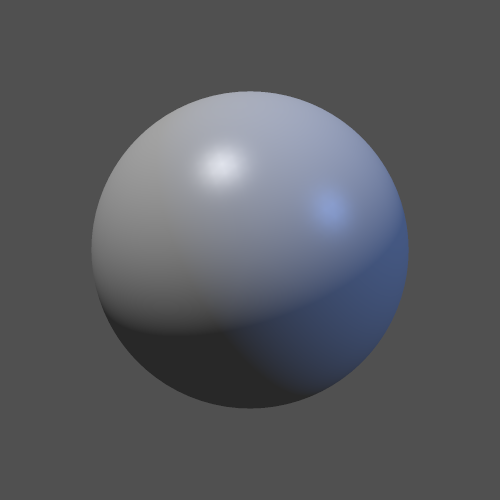
\includegraphics[width=6.5cm]{image/RasterizationIOW/SphereBlinnPhong.png}
\end{Figure}

\xref{fig:Blinn-Phong着色中系数p的影响}展示了Blinn-Phong着色中系数$p$的影响,依次取$p=10,30,100,300$,注意到$p$越大高光的光斑越小。因为根据\xref{fml:Blinn-Phong着色},较大的$p$意味着镜面反射集中在较狭窄的角度范围内。

\begin{Figure}[Blinn-Phong着色中系数$p$的影响;Blinn-Phong着色中系数p的影响]
    \begin{FigureSub}[$p=10$]
        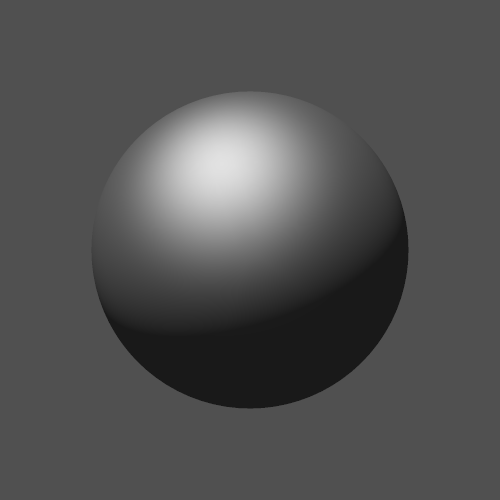
\includegraphics[width=3.53cm]{image/RasterizationIOW/SphereP1.png}
    \end{FigureSub}
    \begin{FigureSub}[$p=30$]
        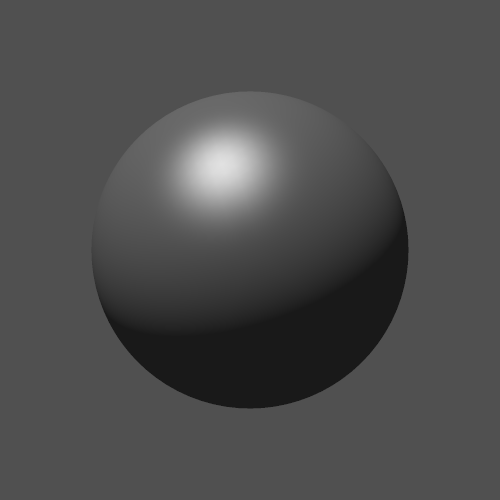
\includegraphics[width=3.53cm]{image/RasterizationIOW/SphereP2.png}
    \end{FigureSub}
    \begin{FigureSub}[$p=100$]
        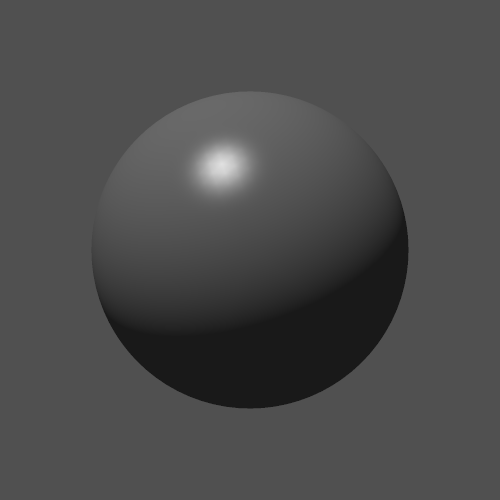
\includegraphics[width=3.53cm]{image/RasterizationIOW/SphereP3.png}
    \end{FigureSub}
    \begin{FigureSub}[$p=300$]
        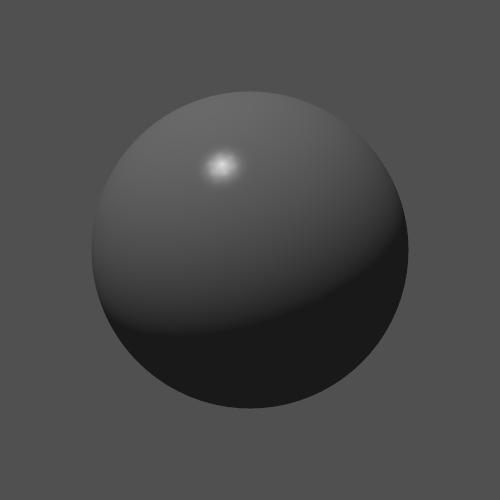
\includegraphics[width=3.53cm]{image/RasterizationIOW/SphereP4.png}
    \end{FigureSub}
\end{Figure}